\documentclass{article}
\usepackage[utf8]{inputenc}
\usepackage{graphicx}

\title{Technical documentation}
\author{Adam Loucký, Vít Knobloch}
\date{May 2021}

\begin{document}

\maketitle

\section{Introduction}
The program is an implementation of PONG game for MZ\_APO kit, it directly accesses the kit's embedded and connected peripherals for output and ssh terminal connection for input. It was developed using remote lab access.

\section{Used technologies}

\begin{itemize}
    \item MZ\_APO kit and provided source code for low level peripheral access and memory mapping
    \item C programming language and GNU Make
    \item Big Blu Button, SSH and WSL2 for lab access
    \item Git and VS Code for source control
    \item Discord for team communication
    \item Overleaf online LaTeX editor for documentation and user manual
\end{itemize}

\section{Building blocks}
The application consists of several building blocks that are interconnected and call each other for their subroutines. The main building blocks and their dependencies are described in the diagram below.
\begin{center}
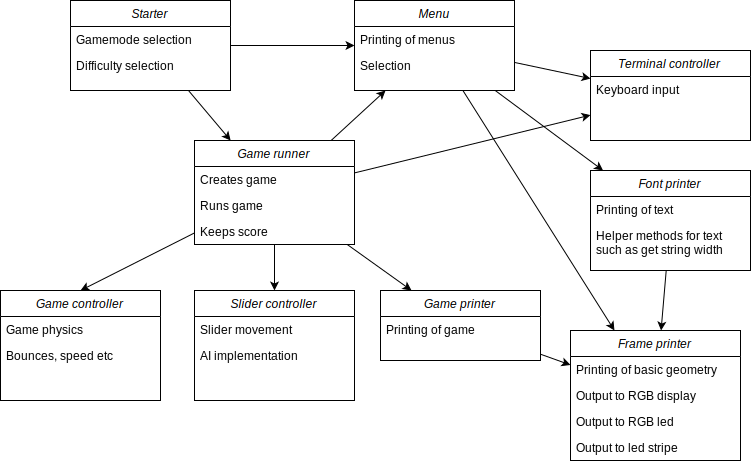
\includegraphics[width=\textwidth]{tech_blocks.png}    
\end{center}
Only the functions which are used by other blocks are defined in the header files. We tried to keep the building blocks as separated as possible.


\end{document}